\cotefile{1}
\scanpage{108}
% ms. line 01
\uline{Genre d'une fonction entière}

% ms. line 02
Il arrive que l'on ait $\sum\frac{1}{|a_n|^{k+1}}<+\infty$
% ms. line 03
pour quelque $k$, (soit $k$ le plus petit entier qui
% ms. line 04
y satisfasse) et de plus que dans la représentation (2),
% ms. line 05
$g(z)$ soit un polynôme --
% ms. line 06
d'ailleurs déterminé à une constante près.

% ms. line 07
Soit $r$ son degré, le plus \deleted{petit} \inserted{grand} des
% ms. line 08
nombres $r,k$ s'appelle le genre de $f(z)$.
% ms. line 08a
\inserted{C'est un nb \uline{entier} $\geq 0$.}

% ms. line 09
Donc si $f(z)$ est de genre $\leq r$, alors on
% ms. line 10
a la formule
% ms. line 11
\[ f(z)=e^{\alpha_0+\alpha_1 z\ldots+\alpha_{\unsure{n|r}}z^{\unsure{n|r}}}\prod_n\left(1-\frac{z}{a_n}\right)e^{\frac{z}{a_n}+\ldots+\frac{z^r}{r a_n^{\unsure{r}}}}\tag*{(3)} \]

% ms. line 12
Dire que $f(z)$ est de genre zéro, signifie
% ms. line 13
que $f(z)$ est de la forme
% ms. line 14-15
\[ \begin{aligned} \vphantom{f(z)}\\[-2pt]\text{avec}\quad \end{aligned}\left\{\begin{aligned} f(z)&=\mathrm c^{\mathrm{te}}\times\prod_n\left(1-\frac{z}{a_n}\right)\\[-2pt] \sum_n\frac{1}{|a_n|}&<+\infty \end{aligned}\right. \tag*{(4)} \]

% ms. line 16
\uline{Ordre d'une fonction entière} \quad Posons $M(r)=\mathop{\rm Sup}_{z\unsure{=|\leq}r}|f(z)|$
% ms. line 17
Puis $\rho=\overline{\lim}\frac{\log\log M(r)}{\deleted{\unsure{z}}\log r}$ \quad $(0\leq\rho\leq+\infty)$, $\rho$ est
% ms. line 18
dit l'ordre de $f(z)$, et $f(z)$ est dite d'ordre
% ms. line 19
fini si $\rho<+\infty$. Cela signifie qu'il existe
% ms. line 20
$k>0$ tel que $|f(z)|\leq e^{(|z|^k)}$. Alors $\rho$
% ms. line 21
est la \deleted{plus petit nombre} \inserted{borne inférieure des} $\sigma>0$ tels que
% archive sheet number: 107
\scanpage{109}
% ms. line 01
\deleted{\unsure{soit|ait}} \inserted{l'on ait} $M(r)\leq e^{(r^\sigma)}$ pour $r$ assez grand.
% Paper watermark, inverted relative to the writing: MADE IN FRANCE (oval); The Best Typewriting Quality.

% ms. line 02
\uline{Théorème 2} (Hadamard-Borel) Si l'ordre $\rho$ de $f(z)$
% ms. line 03
est fini, alors pour tout $\varepsilon>0$, la série
% ms. line 04
\[ \sum{}'\frac{1}{|a_n|^{\rho+\varepsilon}}<+\infty \tag*{(5)} \]
% ms. line 04a
($'$ indique
% ms. line 05
qu'on ne somme pas sur les racines nulles)

% ms. line 06
De plus, on a alors (en supposant $f(0)\ne0$)
% ms. line 07
\[ f(z)=e^{P(z)}\prod_n\left(1-\frac{z}{a_n}\right)e^{\frac{z}{a_n}+\ldots+\frac{z^p}{p a_n^p}} \]
% ms. line 08
où $p\leq\rho$, et $P(z)$ est \deleted{\unsure{un polynôme}} \inserted{un polynôme}
% ms. line 09
de degré $\leq\rho$ \unsure{:|.} en d'autres termes, on
% ms. line 10
a \qquad genre de $f$ $\leq$ ordre de $f$.
% Vertical rule in the left margin alongside the theorem.

% ms. line 11
\uline{Corollaire} \quad Si $\rho<1$, i.e s'il existe un $\unsure{0<\mu|\alpha\mu|\alpha}<1$
% ms. line 12
tel que $M(r)\leq e^{(r^\mu)}$ pour $r$ assez grand,
% ms. line 13
alors $f(z)$ est de genre zéro :
% ms. line 14
\[ f(z)=\mathrm c^{\mathrm{te}}\mathbin{\times}\prod_n\left(1-\frac{z}{a_n}\right)\deleted{\unsure{e^{z/a_n}}} \]

% ms. line 15
\uline{Remarque}. \quad Il est très facile de se convaincre
% ms. line 16
que \qquad ordre de $f$ $\leq$ genre de $f+1$. Donc, si $\omega$ et
% ms. line 17
$g$ sont respectivement le genre et l'ordre, on a
% ms. line 18
\[ \boxed{\omega-1\leq g\leq\omega} \]

% ms. line 19
Comme $\unsure{\gamma|g}$ est entier, il en résulte que $\gamma$
% ms. line 20
est connu dès que $\omega$ l'est, sauf si $\omega$ est
% ms. line 21
entier. En ce cas, on peut avoir $\unsure{p|\gamma|g}=\omega$, ou
% ms. line 21a
$\gamma=\omega-1$.
% archive sheet number: 110
\scanpage{110}
% ms. line 01
P. ex. \deleted{\unsure{si}} $e^{(z^\omega)}$ est une fonction d'ordre $\omega$, de
% Paper watermark as on scan 109: MADE IN FRANCE (oval); The Best Typewriting Quality.
% ms. line 02
genre $\omega$. $\prod_n\left(1-\frac{z}{n^\alpha}\right)$ (où $\alpha>1$) est d'ordre
% ms. line 03
$1$ (sauf erreur) et de genre $0$.

% ms. line 04
Notons que l'ordre du produit de deux
% ms. line 05
fonctions entières est au plus égal au maximum
% ms. line 06
des deux ordres : $\omega(fg)\leq\mathrm{Max}(\omega f,\omega g)$, même
% ms. line 07
chose pour la somme. \deleted{D'où, \unsure{p. ex.} si $f(z)=e^{P(z)}\unsure{\prod}$}
% ms. line 07a
\inserted{l'ensemble des}
% ms. line 08
fonctions entières dont l'ordre est $<\mu$ donné
% ms. line 09
(resp\textsuperscript{t} $\leq\mu$) est une \deleted{\unsure{gr}} algèbre.

% ms. line 10
\uline{Théorème}3 (Hadamard) Soit la fonction entière
% ms. line 11
$f(z)=\sum c_n z^n$. Si $n^\alpha\sqrt[n]{|c_n|}\longrightarrow0$ pour
% ms. line 12
$n$ infini, alors $f$ est au plus de genre $\frac1\alpha$.
% archive sheet number: 111
\scanpage{111}
% ms. line 01
\uline{Proposition} \quad Soit $f(z)$ une fonction entière \deleted{\unsure{satisfaisant}} \deleted{majorée} \inserted{dont}
% ms. line 02
\deleted{\unsure{avec}} \inserted{les} coefficients sont majorés en module par
% ms. line 03
ceux d'une fonction de genre $0$ $h(z)$. Si
% ms. line 04
de plus les racines non nulles $z_i$ de $f(z)$
% ms. line 05
sont telles que $\sum\frac{1}{|z_i|}<+\infty$, $f(z)$ est de
% ms. line 06
genre zéro.

% ms. line 07
\deleted{En effet, $h(z)$ étant d'}

% ms. line 08
Démonstration. On peut supposer
% ms. line 09
que $h(z)$ est de la forme $\unsure{k|\mathrm c|K}^{\mathrm{te}}\times\sum_{i=1}^{\infty}(1+\alpha_i z)$, où
% ms. line 10
les $\alpha_i$ sont $>0$, et $\sum\alpha_i<+\infty$. Comme
% ms. line 11
$h(z)$ est d'\uline{ordre} $\leq1$, il en est de $=$ de
% ms. line 12
$f(z)$, donc on aura
% ms. line 13
\[ f(z)=e^{\alpha+\beta z}z^m\prod_i\left(1-\frac{z}{z_i}\right) \]

% ms. line 14
Il faut montrer que $\beta=0$. On peut supposer
% ms. line 15
pour simplifier $\beta>0$, sinon on remplacerait
% ms. line 16
$f(z)$ par $f(\Theta z)$, avec $\Theta=\beta/|\beta|$. On
% ms. line 17
a alors $\displaystyle |f(z)|=\unsure{K_1^{\mathrm{te}}|K_1|K^{\mathrm{te}}}\times e^{\beta x}|z|^m\prod\left|1-\frac{z}{z_i}\right|$.

% ms. line 18
D'autre part, on sait que \deleted{\unsure{si une}} \inserted{toute} fonction
% ms. line 19
de genre zéro, telle $h(z)$, admet une
% ms. line 20
majoration de la forme $|h(z)|\leq\mathrm C^{\mathrm{te}}\times e^{\varepsilon|z|}$, où
% ms. line 21
on peut prendre $\varepsilon$ arbitraire. \deleted{Si alors on
% ms. line 22
prend $\varepsilon\unsure{<|\leq}\beta$, on aura}
% ms. line 23
\[ \deleted{\deleted{|f(z)|\leq}|z|^m\prod\left|1-\frac{z}{z_i}\right|\leqKe^{\varepsilon|z|}} \]
% ms. line 24
\deleted{avec $z$}
% archive sheet number: 112
\scanpage{112}
% ms. line 01
Notons que si $-\theta\leq\arg z\leq+\theta$, où $\theta$ est
% ms. line 02
un angle arbitraire que nous prendrons une
% ms. line 03
fois pour toutes entre $\frac{\pi}{3}$ et $\pi$, on
% ms. line 04
aura $x\geq c|z|$, où $c$ est une
% ms. line 05
constante $>0$, d'où \deleted{$f(z)\geq$}
\figure{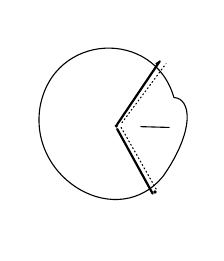
\begin{tikzpicture}[x=1cm,y=1cm,line cap=round]
\draw (0,0) .. controls (-.25,.88) and (-1.53,.83) .. (-1.70,-.12) .. controls (-1.85,-1.05) and (-.7,-1.71) .. (-.13,-.99) .. controls (.27,-.41) and (.22,-.01) .. (0,0);
\draw[thick] (-.72,-.34)--(-.18,.46);
\draw[thick] (-.72,-.40)--(-.27,-1.22);
\draw[densely dotted] (-.66,-.32)--(-.10,.43) (-.67,-.38)--(-.21,-1.19);
\draw[thin] (-.42,-.37)--(-.06,-.38);
\fill (-.73,-.36) circle (.024) (-.21,.43) circle (.025) (-.24,-1.20) circle (.025);
\end{tikzpicture}}
% ms. line 06
\[ |f(z)|\geq e^{c|z|}|z|^m\prod_i\left|1-\frac z{z_i}\right|\qquad\text{qnd }-\theta\leq\arg z\leq+\theta \]

% ms. line 07
D'autre part on a $|f(z)|\leq|h(z)|\leq \mathrm c^{\mathrm{te}}\times e^{\varepsilon|z|}$
% ms. line 08
d'où, en supposant qu'on ait choisi $\varepsilon<c$
% ms. line 09
\[ |z|^m\prod_i\left|1-\frac{z}{z_i}\right|\leq k e^{-\alpha|z|} \]
% ms. line 10
où $\alpha>0$, dès que $-\theta\leq\arg z\leq+\theta$.

% ms. line 11
Posons $g(z)=z^m\prod_i(1-\frac z{z_i})$, notre formule
% ms. line 12
s'écrit \quad \uline{$|g(z)|\leq ke^{-\alpha|z|}$} \quad si $-\theta\leq\arg z\leq+\theta$

% ms. line 13
Montrons qu'une \deleted{telle} inégalité n'est possible
% ms. line 14
pour une fonction $g$ de genre zéro que si elle
% ms. line 15
est \deleted{\unsure{identique}} \inserted{constante}. On a en effet aussi, $g$ étant de genre
% ms. line 16
zéro \qquad $|g(z)|\leq k'e^{\frac{\alpha}{3}|z|}$ \qquad pour l'ensemble
% ms. line 17
Posons $\omega=e^{2i\pi/3}$, et $G(z)=g(z)g(\omega z)g(\omega^{\unsure{2|3}}z)$
% ms. line 18
C'est une fonction entière, et on vérifie
% ms. line 19
aussitôt que, \uline{quel que soit $z$}, on a
% ms. line 20
\[ |G(z)|\leq(ke^{-\alpha|z|})(k'e^{\frac{\alpha}{3}|z|})(k'e^{\frac{\alpha}{3}|z|})=k''e^{-\frac{\alpha}{3}|z|} \]
% ms. line 21
$G(z)$ serait donc bornée, donc une constante.
% ms. line 22
Mais $G(z)=z^{\unsure{3m}}\prod_i\left(1-\frac{z^3}{z_i^3}\right)$, il
% margin note written sideways
% ms. line 23
\margin{\unsure{faudra|faut donc} que l'ens. d'indices $i$ soit vide, et $m=0$, donc que $g(z)$ soit une constante. \unsure{Cela|Cel.|Ceci} signifie que $f(z)=\mathrm C^{\mathrm{te}}e^{\beta z}$, ce qui est incompatible avec $|f(z)|\leq|\deleted{\unsure{g}}h(z)|\leq \mathrm c^{\mathrm{te}}e^{\varepsilon|z|}$.}
% archive sheet number: 113
\scanpage{113}
% ms. line 01
Soit $(\alpha_n)$ une suite \uline{décroissante} \inserted{et convergeant vers zéro} de nombres
% ms. line 02
positifs. Soit $\rho$ la borne inférieure des nombres
% ms. line 03
\deleted{positifs} $s>0$ tels que $(\alpha_n)$ soit majorée par
% ms. line 04
un multiple de la série $\left(\frac{1}{n^{1/s}}\right)$ (et $+\infty$
% ms. line 05
si un tel $s$ n'existe pas) et soit $\sigma$ la
% ms. line 06
borne inférieure des nombres $s>0$, tels que
% ms. line 07
$\sum_n\alpha_n^s<+\infty$. (et $+\infty$ si un tel $s$ n'existe pas)

% ms. line 08
On a aussi $\frac1\rho\deleted{\unsure{\leq}}=\limsup_n\unsure{:}\frac{\log(1/\alpha_n)}{\log n}$. \deleted{$\rho$ et $\sigma$
% ms. line 09
sont resp\textsuperscript{t} les bornes inf. d'ensembles
% ms. line 10
A et B.} -- Le critère de Riemann affirme
% ms. line 11
que \deleted{$\unsure{\rho\leq|\rho\leq\sigma}$} $\sigma\leq\rho$. Mais on a aussi $\rho\leq\sigma$,
% ms. line 12
car on a le

% ms. line 13
\uline{Lemme} \quad Si $s>0$ est tel que $\sum_n\alpha_n^s<+\infty$
% ms. line 14
alors \inserted{$\unsure{\geq}$} \deleted{la suite $(\alpha_n)$ est majorée par un
% ms. line 15
multiple de la suite $\left(\frac1{n^{1/s}}\right)$.} \inserted{$\alpha_n=o\left(\frac1{n^{1/s}}\right)$} ($\alpha_n$ étant décroissant !)

% ms. line 16
Démonstration. On se ramène au cas où $s=1$
% ms. line 17
(en posant $B_n=\alpha_n^s$) \inserted{et à prouver qu'il est impossible que} \deleted{\unsure{sup}} pour une suite
% ms. line 18
strictement croissante d'entiers $n_i$, on \deleted{avait} ait
% ms. line 19
$\alpha_{n_i}\geq\frac1{n_i}$ ; \inserted{en effet, alors} on aurait \quad $\alpha_{n_{i-1}+1}+\alpha_{n_{i-1}+2}+\ldots+\alpha_{\unsure{n_i|n}}\geq\frac{n_i-n_{i-1}}{n_i}$
% ms. line 20
soit $\varepsilon_i$ ce second membre, $\sum\varepsilon_i$ est donc
% ms. line 21
convergente, et on a $n_i(1-\varepsilon_i)=n_{i-1}$, d'où $n_i=\frac{n_{i-1}}{1-\varepsilon_i}$
% ms. line 22
$\displaystyle =\frac{n_{i-2}}{(1-\varepsilon_i)(1-\varepsilon_{i-1})}\ldots=\frac1{(1-\varepsilon_{\unsure{1|i}})\ldots(1-\varepsilon_{\unsure{n|i}})}\leq\frac1{\prod_1^\infty(1-\varepsilon_k)}$, la suite
% ms. line 23
des $n_i$ est donc majorée, et s'arrête donc.
% archive sheet number: 114
\scanpage{114}
% ms. line 01
\uline{Supposons} maintenant que l'on ait $\sum\alpha_i<+\infty$,
% ms. line 02
posons $f(z)=\prod_1^\infty(1+\alpha_i z)$. Alors $\rho$ est aussi
% ms. line 03
l'ordre de la fonction entière, i.e
% ms. line 04
\[ \rho=\limsup_{0<r\to\infty}\frac{\log(\log f(r))}{\log r} \]

% ms. line 05
En effet, on sait que $\rho$ est $\leq$ ordre de la
% ms. line 06
fonction $f(z)$, \deleted{\unsure{et}} \unsure{montrons|démontrons} \unsure{la|le} contraire. On est
% ms. line 07
ramené à montrer que \deleted{le produit} dans le
% ms. line 08
cas où on a $\alpha_n=\frac1{n^\beta}$, on a
% ms. line 09
$\displaystyle \limsup_{0<r\to\infty}\frac{\log\log f(r)}{\log r}\leq\frac1\beta$ \quad (\unsure{en somme on a|on verra|on sait} en fait $=\frac1\beta$)

% ms. line 10
En effet, on a
% ms. line 11
\[ f(r)=\prod_1^{\unsure{\nu|v}}\left(1+\frac1{n^\beta}r\right)\prod_{\nu+1}^{\infty}\left(1+\frac1{n^\beta}r\right) \]
% ms. line 12
le deuxième facteur est $\leq e^{R(\nu)r}$
% ms. line 13
avec $\displaystyle R(\nu)=\sum_{\nu+1}^\infty\frac1{n^\beta}\leq\int_\nu^\infty\frac{\unsure{dx|du}}{x^\beta}=\frac1{\beta-1}\frac1{\nu^{\beta-1}}$
% ms. line 14
Prenons $\nu$ tel que $r\frac1{\nu^{\beta-1}}\leq r^{\frac1\beta}$, i.e $\nu\geq r^{\frac1\beta}$
% ms. line 15
de façon précise, $\nu=[r^{\frac1\beta}]+1$. Alors, $e^{R(\nu)r}$
% ms. line 16
sera une \uline{fonction de $r$} d'ordre $\leq\frac1\beta$. Il
% ms. line 17
suffit de le vérifier pour le produit $\prod_1^\nu(1+\frac1{n^\beta}r)$
% ms. line 18
$\leq(1+r)^\nu=e^{\nu\log(1+r)}$, qui est manifestement
% ms. line 19
d'ordre $\leq\frac1\beta$.

% ms. line 20
Rappelons que si on pose $f(\unsure{z|r})=\sum a_n z^n$,
% ms. line 21
\deleted{\unsure{dans}} et $B(r)=\mathop{\rm Sup}_n(a_n r^n)$, alors on
% ms. line 22
a aussi \qquad ordre \unsure{à|de} $f=\limsup_{r\to\infty}\frac{\log\log B(r)}{\log r}$
% archive sheet number: 115
\scanpage{115}
% ms. line 01
Soit $f(z)=\prod_1^\infty(1+\lambda_iz)$ une fonction entière
% ms. line 02
de \uline{genre} $1$, posons $\alpha_i=|\lambda_i|$, $F(z)=\prod_{\unsure{1|i}}^\infty(1+\alpha_i z)$.
% ms. line 03
Alors \uline{$f$ et $F$ ont $=$ ordre} (qui s'exprime donc
% ms. line 04
aussi en fonction de la suite des $|\alpha_i|$). En effet,
% ms. line 05
l'ordre de $f\leq$ ordre de $F$ (évident). D'autre
% ms. line 06
part, ordre de $F=$ ordre de la suite des $|\alpha_i|$
% ms. line 07
(voir ci-dessus) $\leq$ ordre de $f$ (th. de Hadamard).
\begin{center}\rule{1.5cm}{0.4pt}\end{center}

% ms. line 08
On peut parler de l'ordre d'un ensemble \inserted{dénombrable} de
% ms. line 09
nombres complexes, \deleted{indépendamment de} \inserted{$=$ \unsure{non} \unsure{rangés|compris} en suite :}
% ms. line 10
on prend la borne inf. des $s>0$ tels que
% ms. line 11
$\sum|z_i|^s<+\infty$. Suite à décroissance rapide $=$
% ms. line 12
d'ordre zéro.

% ms. line 13
Ordre d'une suite dans un espace de Banach,
% ms. line 14
ou de Fréchet. (deux définitions, suivant qu'on
% ms. line 15
prend sommabilité forte, ou sommabilité absolue)

% ms. line 16
Ordre d'une partie bornée (\deleted{plus petit} \inserted{borne inférieure} des
% ms. line 17
$s>0$ tels que la partie soit contenue dans l'enveloppe
% ms. line 18
convexe cerclée fermée d'une suite d'ordre $s$)
% archive sheet number: 116
\scanpage{116}
% ms. line 01
Soit $(r_{\unsure{\nu|v}})$ suite croissante de nombres \deleted{\unsure{positifs}} $>0$, $\to\infty$
% ms. line 02
soit $n(r)$ le nombre des indices $\nu$ tels que
% ms. line 03
$r_\nu\leq r$, on a, pour $0\leq a\leq b<+\infty$, et $\alpha>0$
% ms. line 04
\[ \boxed{\displaystyle \sum_{\substack{\nu\\(a<r_\nu<b)}}\frac1{r_\nu^\alpha}=\left(\frac{n(b-0)}{b^\alpha}-\frac{n(a+0)}{a^\alpha}\right)+\alpha\int_a^b\frac{n(r)\,dr}{r^{\alpha+1}}}\tag*{(1)} \]
% ms. line 05
(car le premier membre est égal à $\int_{\unsure{a_0|r_0|a}}^b r^{-\alpha}\,dn(r)$,
% ms. line 06
et on intègre par parties)

% ms. line 07
\uline{Proposition} \quad $\displaystyle \sum_\nu\frac1{r_\nu^\alpha}<+\infty\ \Longleftrightarrow\ \int_0^\infty\frac{n(r)\,dr}{r^{\alpha+1}}\unsure{\leq|<}+\infty$
% ms. line 08
alors $\frac{n(r)}{r^\alpha}\to0$ pour $r\to\infty$, et on a
% ms. line 09
\[ \boxed{\displaystyle \sum_{\substack{\nu\\(r_\nu>a)}}\frac1{r_\nu}=-\frac{n(a+0)}{a^\alpha}+\alpha\int_a^\infty\frac{n(r)\,dr}{r^{\alpha+1}}}\tag*{\unsure{(1)|(1\textquotesingle)}} \]
% Vertical stroke in the left margin alongside the proposition.

% ms. line 10
\deleted{$\leftarrow$ \unsure{si} $\sum_\nu\frac1{r_\nu^\alpha}<+\infty$, on a $\frac{n(r)}{r^\alpha}\leq M$ pour \unsure{tout} $r$
% ms. line 11
où $M=$ constante}
% ms. line 12
En effet, (1) s'écrit, pour $a=0$, \deleted{\unsure{comme}}
% ms. line 13
\[ \sum_{r_\nu<b}\frac1{r_\nu^{\unsure{\alpha|\nu}}}=\frac{n(b-0)}{b^\alpha}+\alpha\int_0^b\frac{n(r)\,dr}{r^{\alpha+1}}\tag*{\textcircled{\scriptsize 1 bis}} \]
% ms. line 14
d'où suit que si \deleted{\unsure{pour un} $b$} $\sum_\nu\frac1{r_\nu^\alpha}$ est
% ms. line 15
convergente, il en est de $=$ de $\int_0^\infty\frac{n(r)\,dr}{r^{\alpha+1}}$
% ms. line 16
Réciproquement, si $\int_{\unsure{0}}^\infty\frac{n(r)\,dr}{r^{\alpha+1}}<+\infty$ alors il
% ms. line 17
existe $M>0$ et une suite croiss. de $b_i\to\infty$
% ms. line 18
de nbs tels que $\frac{n(b_i)}{b_i^\alpha}\leq M$ ; \unsure{p.} on a donc
% ms. line 19
$\displaystyle \sum_{r_\nu<b_i}\frac1{r_\nu^\alpha}\leq M+\alpha\int_0^\infty\frac{n(r)\,dr}{r^{\alpha+1}}$, d'où $\displaystyle \tikz[baseline=(a.base)]{\node[inner sep=1pt] (a) {$\displaystyle\sum_{\unsure{i|\nu}}\frac1{r_i^\alpha}$};\draw ([yshift=3pt]a.south west)--(a.south west)--(a.south east)--([yshift=3pt]a.south east);}<+\infty$.
% archive sheet number: 117
\scanpage{117}
% ms. line 01
Montrons qu'alors $\frac{n(r)}{r^\alpha}\to0$ ; si en effet on avait
% ms. line 02
$\frac{n(b_i)}{b_i^\alpha}>\varepsilon$ pour des $b_i\to+\infty$, on aurait
% ms. line 03
$n(b_i)-n(b_{i-1})\geq\varepsilon\lambda_i^\alpha-M\lambda_{i-1}^\alpha$ d'où
% ms. line 04
\[ \sum_{\substack{\unsure{\nu|v}\\b_{i-1}<r_\nu\leq b_i}}r_\nu^{-\alpha}\geq\big(n(b_i)-n(b_{i-1})\big)\lambda_i^{-\alpha}\geq\varepsilon-M\left(\frac{\lambda_{i-1}}{\lambda_i}\right)^\alpha \]
% ms. line 05
on peut supposer $M\left(\frac{\unsure{b_{i-1}|\lambda_{i-1}}}{\lambda_i}\right)^\alpha\leq\frac{\varepsilon}{2}$ pour tout $i$,
% ms. line 06
d'où $\sum_{b_{i-1}<r_\nu\leq b_i}r_\nu^{-\alpha}\geq\frac{\varepsilon}{2}$, \deleted{d'où $\sum$} ce
% ms. line 07
qui est contradictoire.

% ms. line 08
Si alors on fait $b\to\infty$ dans (1 bis), on
% ms. line 09
obtient (2).

% ms. line 10
\deleted{\illegible{1}} Des résultats analogues seraient obtenus si
% ms. line 11
on considérait les sommes $\sum_\nu\lambda(r_\nu)$, où
% ms. line 12
$\lambda$ est fonction définie sur $R^{+*}$, continûment
% ms. line 13
différentiable, \inserted{décroissante,} et tendant vers zéro
% ms. line 14
\deleted{\unsure{pour}} à l'infini\unsure{\}} : Alors
% ms. line 15
\[ \boxed{\displaystyle \sum_\nu\lambda(r_\nu)<+\infty\ \Longleftrightarrow\left\{\begin{aligned}&\int_0^\infty n(r)[-\lambda'(r)]\,dr<+\infty\\[-2pt]&\deleted{\text{et }\lambda(r)n(r)\ \text{\unsure{reste borné}}}\end{aligned}\right.} \]
% ms. line 16
et alors $\lambda(r)n(r)\to0$ pour $r$ infini, et
% ms. line 17
on a \quad $\displaystyle\sum_{r_\nu>a}\lambda(r_\nu)=-\lambda(\deleted{\unsure{b}}a)n(a+0)+\int_a^\infty n(r)(-\lambda'(r))\,dr\deleted{\unsure{]}}$
% ms. line 18
\deleted{\unsure{Ceci}}
% archive sheet number: 118
\scanpage{118}
% ms. line 01
Supposons maintenant que $(r_{\unsure{\nu|v}})$ soit la suite des
% ms. line 02
modules des zéros d'une fonction entière $f(z)$.
% ms. line 03
On aura $\displaystyle 2\pi n(r)=\int_0^{\deleted{\unsure{a}}2\pi}\frac{f'(re^{i\varphi})}{f(re^{i\varphi})}re^{i\varphi}\,d\varphi$, d'où
% ms. line 04
\[ \begin{aligned} 2\pi\int_a^b n(r)\mu(r)\,dr
&=\int_a^b\int_0^{2\pi}\frac{f'(re^{i\varphi})}{f(re^{i\varphi})}e^{i\varphi}\cdot\deleted{d\varphi}\ r\mu(r)\,dr\,d\varphi\\
% ms. line 05
&=\int_0^{2\pi}d\varphi\int_a^b\underbrace{\frac{f'(re^{i\varphi})}{f(re^{i\varphi})}e^{i\varphi}\,dr}_{d_r\log f(re^{i\varphi})}\ (r\mu(r)) \end{aligned} \]
% ms. line 06
\[ \int_a^b=\left[r\mu(r)\log f(re^{i\varphi})\right]_a^b-\int_a^b\log f(re^{i\varphi})\,d(r\mu(r)) \]
% ms. line 07
(en supposant $\mu(r)$ continûment différentiable)

% ms. line 08
-- On choisit brutalement la détermination
% ms. line 09
principale du logarithme -- pas de trouble,
% ms. line 10
car les intégrales \deleted{\unsure{si elles ont|simplement}} doubles
% ms. line 11
qui interviennent sont convergentes)
\figure{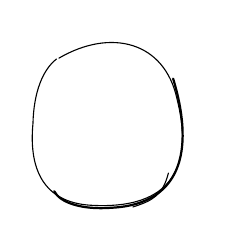
\begin{tikzpicture}[x=1cm,y=1cm,line cap=round]
\draw (.23,1.81) .. controls (.88,2.19) and (1.57,2.03) .. (1.73,1.29) .. controls (1.98,.29) and (1.52,-.10) .. (.67,-.06) .. controls (.08,-.04) and (-.16,.34) .. (-.10,.98) .. controls (-.09,1.37) and (.02,1.66) .. (.20,1.80);
\draw[thick] (1.68,1.55) .. controls (1.93,.73) and (1.85,-.04) .. (.90,-.09) .. controls (.51,-.12) and (.24,-.02) .. (.17,.12);
\draw (1.62,.35) .. controls (1.55,.07) and (1.42,.00) .. (1.17,-.08);
\end{tikzpicture}}
% ms. line 12
D'où, en substituant, intervertissant les signes $\int\!\int$, et
% slanted
% ms. line 12a
\margin{en prenant les parties réelles}
% ms. line 13
\[ \boxed{\displaystyle \deleted{2\pi}\int_{\unsure{a}}^b n(r)\mu(r)\,dr=\left[r\mu(r)V(r)\right]_a^b-\int_a^b V(r)\,d(r\mu(r))} \]
% ms. line 14
où \qquad \uline{$\displaystyle V(r)=\frac1{2\pi}\int_0^{2\pi}\log|f(re^{i\varphi})|\,d\varphi$}
% ms. line 15
Prenons $\mu(r)=-\lambda'(r)$, on obtient \enspace $(0<a<b<+\infty$
% ms. line 16
\[ \boxed{\begin{aligned}\sum_{\substack{\nu\\a<r_\nu<b}}\lambda(r_\nu)^{\deleted{\unsure{\alpha}}}&=\lambda(b)n(b-0)-\lambda(a)n(a+0)+[r\mu(r)V(r)]_a^b\deleted{\unsure{+\int V(r)\,d(r\mu)|+\int}}\\
% ms. line 17
&\qquad+\int_a^b V(r)\,d(r\lambda'(r))\end{aligned}} \]
% archive sheet number: 119
\scanpage{119}
% ms. line 01
(Si $r^2\mu(r)\to0$ pour $r\to0$, et $|f(0)|=1$, on a
% ms. line 02
\[ \sum_{r_{\unsure{\nu|v}}<b}\lambda(r_\nu)=\lambda(b)n(b-0)\deleted{\unsure{+}}-b\lambda'(b)V(b)+\int_0^b V(r)\,d(r\lambda'(r))\quad\big) \]

% ms. line 03
Comme $|V(r)|\leq M(r)=\mathop{\rm Sup}_{|z|\unsure{=|:}r}|f(z)|$, on obtient une
% ms. line 04
majoration de \deleted{$\sum\lambda(r_\nu)$} $\int_{\unsure{a|0}}^b n(r)\mu(r)\,dr$ en fonction
% ms. line 05
de $M(r)$
% archive sheet number: 120
\scanpage{120}
% ms. line 01
\uline{Sur une certaine fonction holomorphe \deleted{\unsure{de variable|définie}} \inserted{sur l'}espace de Banach $l^1$.}

% ms. line 02
Soit, pour $\lambda=(\lambda_i)\in l^1$ et tout entier $n>0$
% ms. line 03
\[ \alpha_n(\lambda)=\sum_{i_1<\ldots<i_n}\lambda_{i_1}\ldots\lambda_{i_n} \]
% ms. line 03a
On a
% ms. line 04
\[ \alpha_n(\lambda)\leq\frac{\|\lambda\|_1^n}{n!} \]
% ms. line 05
les $\alpha_n(\lambda)$ sont les coefficients de la fonction entière
% ms. line 06
de genre zéro
% ms. line 07
\[ f(\unsure{\lambda|n|z})=\prod_{\unsure{1|i}}(1+\lambda_i z) \]
% ms. line 08
et on obtient, à un facteur constant près, les
% ms. line 09
coefficients les plus généraux d'une fonction entière
% ms. line 10
de genre zéro.

% ms. line 11
\uline{Proposition} Pour tout $\lambda\in l^1$, la série $\sum_0^\infty n!\alpha_n(\lambda)$
% Vertical rule beside the proposition.
% ms. line 12
est absolument convergente, soit $S(\lambda)$ sa somme.
% ms. line 13
La fonction $\lambda\to S(\lambda)$ est holomorphe au voisinage
% ms. line 14
de $0$, avec un rayon de convergence égal à $1$,
% ms. line 15
\deleted{\unsure{ce qui fait que ses|ce qui fait que sur}} \inserted{et ses restrictions} aux sous-espaces vectoriels
% ms. line 16
complexes de $\mathrm{dim}$ finie sont holomorphes.
% ms. line 17
Cependant, \deleted{elle} cette fonction n'est pas bornée
% ms. line 18
dans la boule unité de $l^1$, et n'est par
% ms. line 19
suite pas une fonction entière de $\lambda$.

% ms. line 20
\uline{Corollaire} On a \inserted{pour $\lambda\in l^1$} $\sqrt[n]{n!|\alpha_n(\lambda)|}\to 0$,
% Vertical rule beside the corollary.
% ms. line 21
$\sqrt[n]{|\alpha_n(\lambda)|}=o\left(\frac{1}{n}\right)$, $\alpha_n(\lambda)=\frac{\varepsilon_n^n}{n!}$ avec $\varepsilon_n\to 0$
% ms. line 22
Si $\sum a_nz^n$ est une fonction entière de
% ms. line 23
genre zéro, la suite des $a_n$ jouit
% ms. line 24
des $=^{\mathrm s}$ propriétés.

% ms. line 25
En effet, $\sqrt[n]{n!|\alpha_n(\lambda)|}\to 0$ exprime que
% archive sheet number: 121
\scanpage{121}
% ms. line 01
\[ \sum n!\alpha_n(\lambda z)=\sum n!\alpha_n(\lambda)z^n \]
% ms. line 01a
converge
% ms. line 02
quel que soit $z$. Les deux \inserted{autres} relations
% ms. line 03
\deleted{\unsure{sont}} sont une autre façon d'exprimer la première,
% ms. line 04
-- en tenant compte de la formule de
% ms. line 05
Stirling $\sqrt[n]{n!}\sim\frac{n}{e}$ --.

% ms. line 06
Démonstration de la proposition. On peut
% ms. line 07
supposer les $\lambda_i>0$ \inserted{et \uline{décroissants}} $\unsure{]|;|.}$ soit alors $f(z)=\prod(1+\lambda_i z)$
% ms. line 08
\deleted{\unsure{une fonction}}, \inserted{$=\sum\alpha_n\deleted{(\lambda)}z^n$} \inserted{(où on pose $\alpha_n=\alpha_n(\lambda)$)} on a, \deleted{\unsure{en vertu de}} l'inégalité
% ms. line 09
de Cauchy
% ms. line 10
\[ \alpha_n\leq\frac{M(R)}{R^{n+1}}\qquad\text{pour tout }R>0 \]
% ms. line 11
où $M(R)$ est le maximum de $|f(z)|$ sur la
% ms. line 12
circonférence $|z|=R$, \unsure{d'où|d'ici|donc} $M(R)=\prod(1+\lambda_iR)$.
% ms. line 13
\deleted{Soit} On a donc
% ms. line 14
\[ \alpha_n\leq\left(\frac1R+\lambda_1\right)\ldots\left(\frac1R+\lambda_{n+1}\right)\prod_{i=n+2}^{\infty}(1+\lambda_i R) \]
% ms. line 15
\deleted{un facteur} \inserted{Or} $\prod_{i=n+2}^{\infty}(1+\lambda_i R)\leq e^{\rho_{n+1}R}$, où
% ms. line 16
$\rho_{n+1}=\sum_{k=n+2}^{\infty}\lambda_k$. faisons $R=\frac{n+1}{\rho_{n+1}}$, on obtient
% ms. line 17-18
\[ \begin{aligned} \alpha_n&\leq\left(\frac{\rho_{n+1}}{n+1}+\lambda_1\right)\ldots\left(\frac{\rho_{n+1}}{n+1}+\lambda_{n+1}\right)e^n \deleted{\unsure{\leq(\frac{\rho_1}{1}+\lambda_1)\ldots(\rho_{n+1}}}\\ &\leq\left(\frac{\unsure{\rho_1|\rho_2}}{1}+\lambda_1\right)\left(\frac{\rho_2}{2}+\lambda_2\right)\ldots\left(\frac{\rho_{n+1}}{n+1}+\lambda_{n+1}\right)e^n \end{aligned} \]
% ms. line 19
Or, \deleted{\unsure{comme les}} \inserted{les} $\lambda_i$ \deleted{\unsure{sont}} \unsure{étant|formant} décroissants et leur
% ms. line 20
suite sommable, on a $\lambda_n=\unsure{o|O}(\frac1n)$, d'autre part on
% ms. line 21
a \deleted{$\unsure{\rho_n\leq 0|\rho_n\to 0}$} $\frac{\rho_n}{n}=\uline{o}(\frac{1}{n})$, d'où $\frac{\rho_n}{n}+\lambda_n\leq\frac{\varepsilon_{n+1}}{n}$, où $\varepsilon_n\to0$
% ms. line 22
\[ \alpha_n\leq\frac{\varepsilon_{\unsure{1|0}}\varepsilon_2\ldots\varepsilon_{n+1}}{(n+1)!}e^n\qquad\text{où }\varepsilon_i\to0. \]
% ms. line 22a
D'où
% archive sheet number: 122
